\documentclass[aspectratio=169]{beamer}
\usetheme{Madrid}
\usecolortheme{seahorse}
\usepackage{graphicx}
\usepackage{booktabs}
\usepackage{amsmath}
\usepackage{xcolor}

\title[Chapter 3: Scatterplots \& Correlation]{\textbf{Chapter 3: Scatterplots and Correlation}}
\subtitle{School of Mathematical and Computational Sciences \\ University of Prince Edward Island}
\author{Ali Raisolsadat}
\date{Part I: Exploring Data}

\begin{document}

% =============================================================
% PART I: BIVARIATE DATA & VARIABLES
% =============================================================

% SLIDE 1
\begin{frame}
  \titlepage
\end{frame}

% SLIDE 2
\begin{frame}{Bivariate Data}
\begin{itemize}
	\item In Chapters 1 and 2, we examined one variable at a time. For example, we might study the distribution of test scores or household incomes. This is called \textbf{univariate data analysis}.
	\item Many statistical questions involve studying how two variables are related.
	\item For example, we might ask whether study time is related to exam score or whether temperature is related to electricity use.
	\item When two quantitative variables are measured on the same individual or observational unit, we have \textbf{bivariate data}.
\end{itemize}
\end{frame}

% SLIDE 3
\begin{frame}{Explanatory vs. Response Variables}
When studying the relationship between two variables, it is useful to identify the role of each variable.
\vspace{0.3cm}
\begin{itemize}
	\item \textbf{Response Variable ($y$):} The outcome variable that we want to explain or predict.
	\item \textbf{Explanatory Variable ($x$):} The variable that may help explain or predict changes in the response variable.
\end{itemize}
\vspace{0.3cm}
\begin{block}{Note on Terminology}
The explanatory variable is sometimes called the \emph{predictor} or \emph{independent variable}. The response variable is sometimes called the \emph{dependent variable} or \emph{target variable}.
\end{block}
\end{frame}

% SLIDE 4
\begin{frame}{Assigning Variables}
 \textbf{Ex 3.1: Enzyme Activity and Temperature} \\
 Students run an enzyme reaction at different water bath temperatures and measure how much oxygen gas is produced.
 \begin{table}
 \centering
\scriptsize
\begin{tabular}{lll}
\toprule
\textbf{Variable} & \textbf{Measurement} & \textbf{Biological Role} \\
\midrule
Explanatory ($x$) & Temperature ($^\circ$C) & Students manipulate this to drive the reaction speed. \\
Response ($y$) & Oxygen Gas (mL) & The biological outcome being measured. \\
\bottomrule
\end{tabular}
\end{table}
\vspace{0.2cm}
\textbf{Ex 3.2: Forest Ecology and Plant Growth} \\
An ecologist measures the percentage of open sky (canopy cover) and the height of the tallest fern in 50 forest plots.
\begin{table}
 \centering
\scriptsize
\begin{tabular}{lll}
\toprule
\textbf{Variable} & \textbf{Measurement} & \textbf{Biological Role} \\
\midrule
Explanatory ($x$) & Canopy Open Sky (\%) & The physical environment is the underlying cause. \\
Response ($y$) & Fern Height (cm) & The biological growth response. \\
\bottomrule
 \end{tabular}
 \end{table}
\end{frame}

% SLIDE 5
\begin{frame}{Context Matters}
  \textbf{Ex 3.3: Beer and Blood Alcohol} \\
  Student volunteers drank different amounts of beer and a police officer measured their blood alcohol concentration (BAC). 
  \begin{itemize}
      \item Explanatory ($x$): Number of beers consumed
      \item Response ($y$): Percent alcohol in blood
  \end{itemize}
  \vspace{0.3cm}
  \textbf{Ex 3.4: Height} \\
	Statistics Canada's Canadian Health Measures Survey (CHMS) collects health information and physical measurements from Canadians, including height, age and sex. When the goal is simply to describe these measurements, there may be no explanatory or response variable. \\
	\emph{However}, if a researcher uses the data to study how height changes with age, then Age would be the \textbf{Explanatory} variable ($x$) and Height would be the \textbf{Response} variable ($y$).
\end{frame}

% =============================================================
% PART II: SCATTERPLOTS
% =============================================================

% SLIDE 6
\begin{frame}{Scatterplots}
  Once we have identified our explanatory ($x$) and response ($y$) variables, the most effective way to display their relationship is a \textbf{scatterplot}.
  \vspace{0.3cm}
  
  \textbf{Rules for Building a Scatterplot:}
  \begin{enumerate}
    \item Plot the \textbf{Explanatory Variable on the horizontal ($x$) axis}.
    \item Plot the \textbf{Response Variable on the vertical ($y$) axis}.
    \item Each individual appears as exactly \textbf{one dot} on the graph, located at the intersection of their $x$ and $y$ values.
  \end{enumerate}
\end{frame}

% SLIDE 7
\begin{frame}{Examining a Scatterplot}
  \begin{block}{What to look for}
    In any graph of data, look for the overall pattern and for striking deviations from that pattern.
  \end{block}
  \vspace{0.2cm}
  We describe the overall pattern of a scatterplot using four characteristics:
  \begin{itemize}
    \item \textbf{Form:} Is the relationship \emph{Linear} (straight line) or \emph{Non-Linear} (curved, U-shaped)?
    \item \textbf{Direction:} \emph{Positive association} (slopes upward) or \emph{Negative association} (slopes downward).
    \item \textbf{Strength:} How tightly do the points cluster around the underlying form? (\emph{Strong, moderate or weak}).
    \item \textbf{Outliers:} Are there points that fall far outside the overall cloud?
  \end{itemize}
\end{frame}

% SLIDE 8
\begin{frame}{Example 3.5: Linear Relationships}
\footnotesize
\begin{columns}[c]
\begin{column}{0.48\textwidth}
\textbf{Context:} Researchers are studying whether the surface charge of a Lipid Nanoparticle (LNP) is related to how efficiently it enters cells. They prepare several LNP formulations with different surface charges and measure the percentage of particles taken up by cells. Each point represents one LNP formulation.
\begin{itemize}
	\item \textbf{Explanatory variable ($x$):} LNP surface charge
	\item \textbf{Response variable ($y$):} Cellular uptake efficiency
	\item \textbf{Form:} Linear
	 \item \textbf{Direction:} Positive
	\item \textbf{Strength:} Moderate-to-Strong
	\item \textbf{Outliers:} None apparent
\end{itemize}
\end{column}
\begin{column}{0.5\textwidth}
	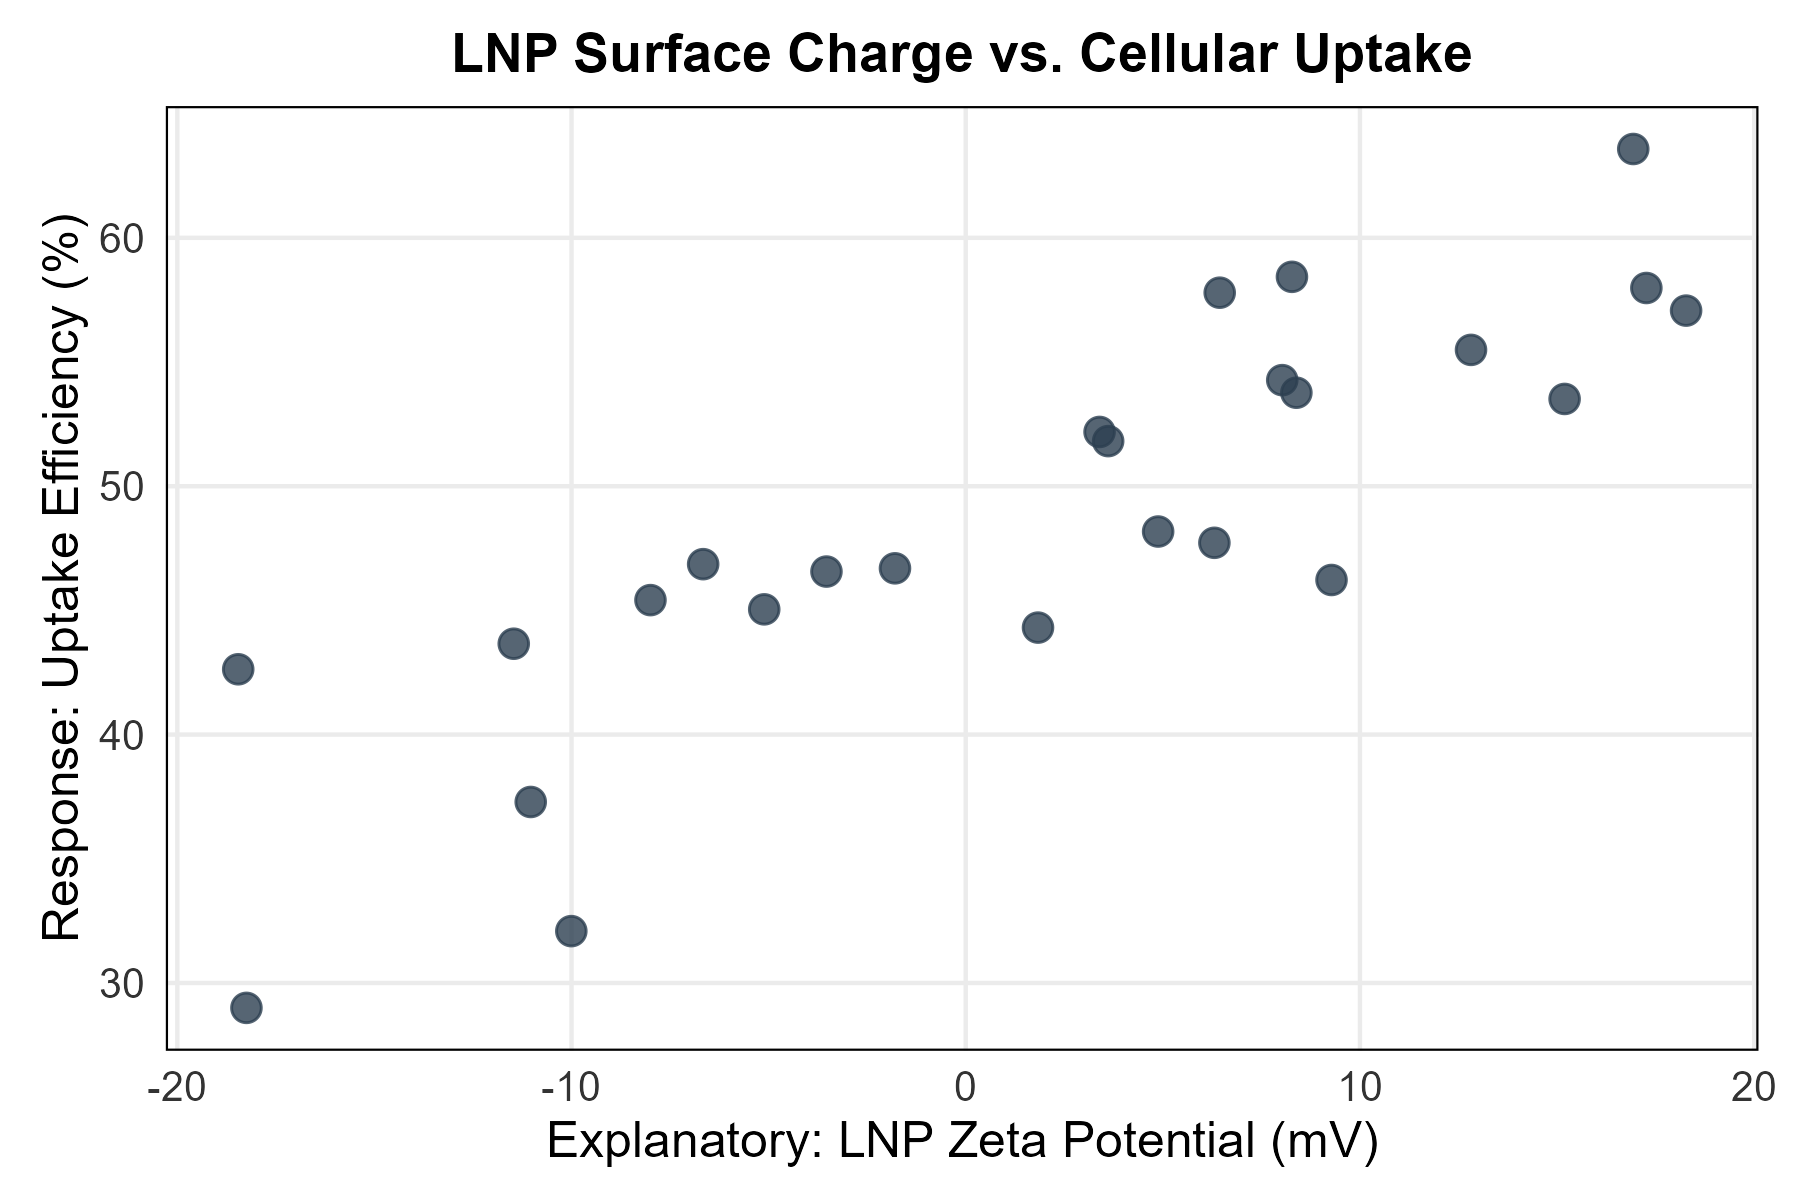
\includegraphics[width=\textwidth]{fig_ch3_scatterplot.png}
\end{column}
\end{columns}
\end{frame}

% SLIDE 9
\begin{frame}{Example 3.6: Non-Linear Relationships}
\footnotesize
 \begin{columns}[c]
 \begin{column}{0.5\textwidth}
	 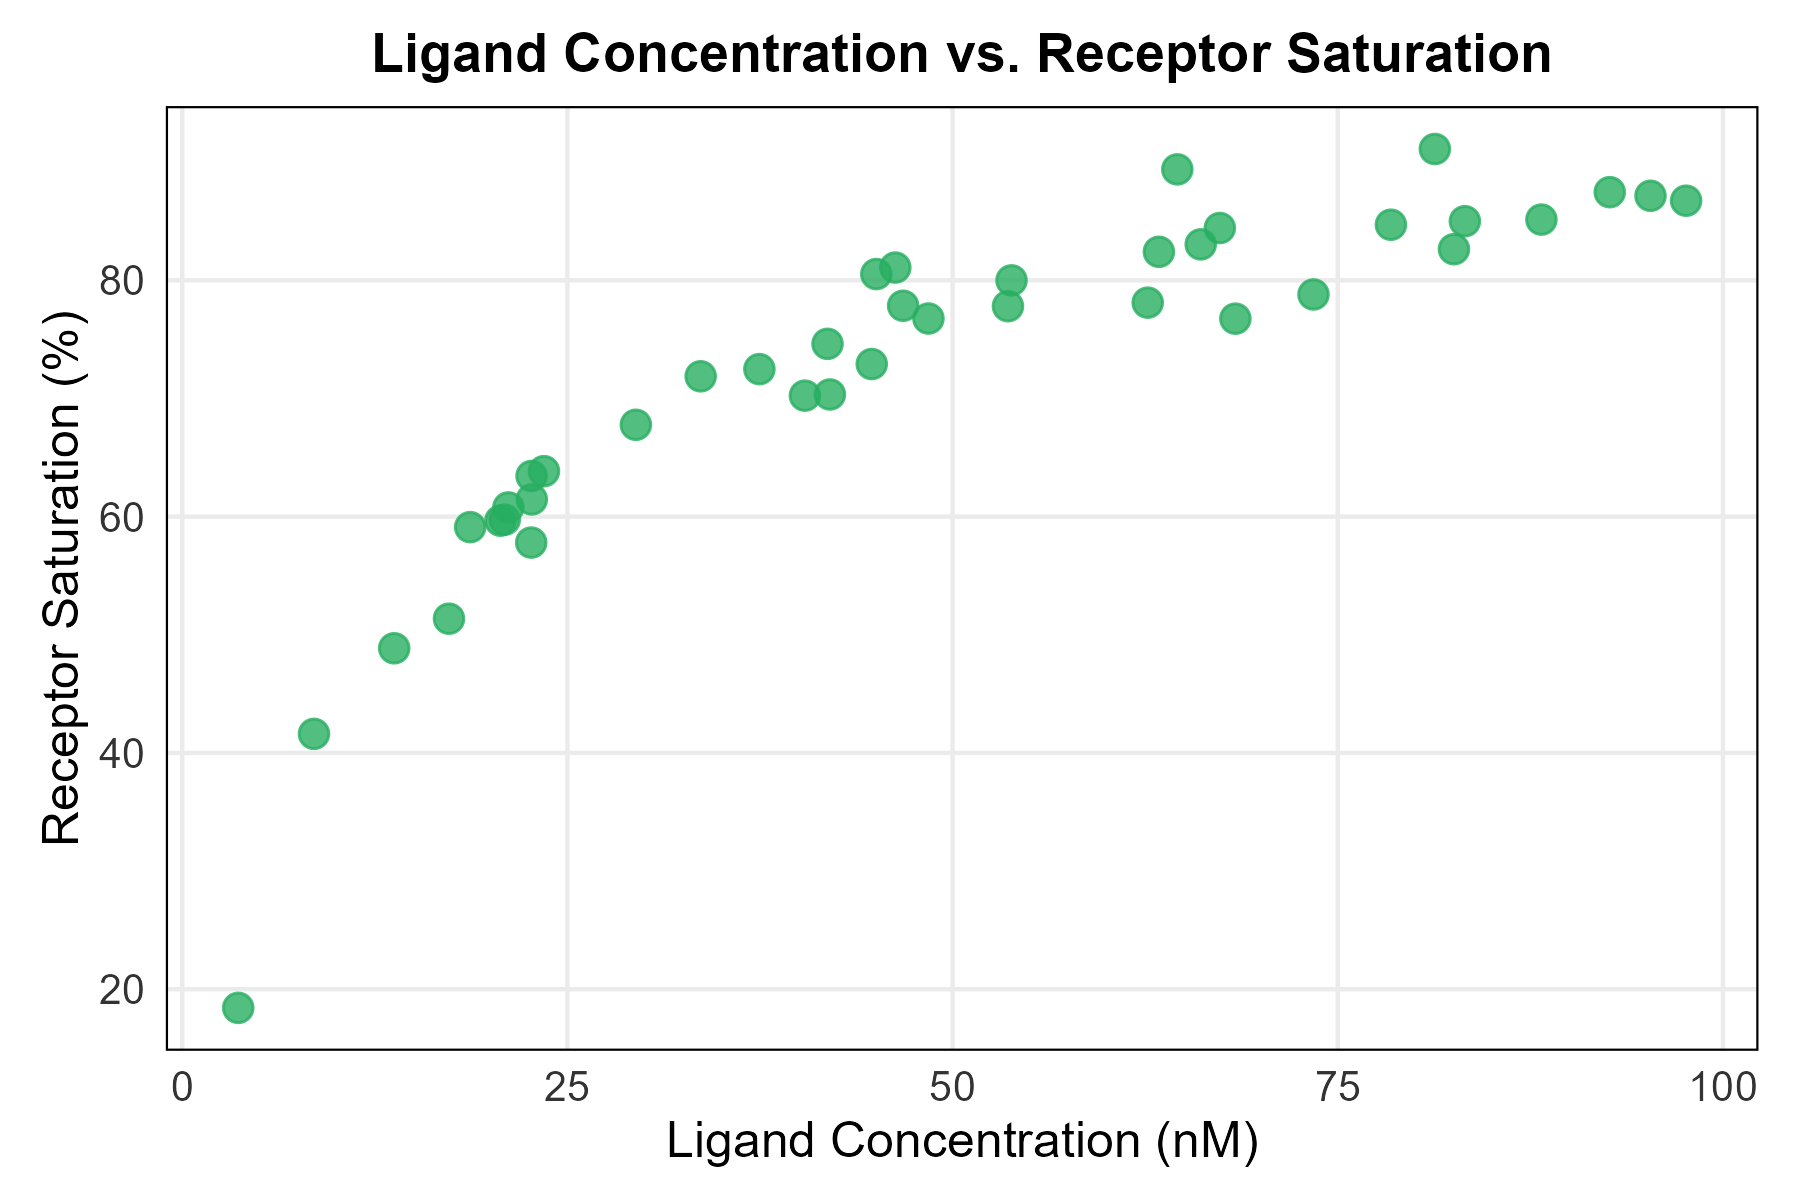
\includegraphics[width=\textwidth]{fig_ch3_nonlinear.png}
 \end{column}
 \begin{column}{0.48\textwidth}
 \textbf{Context:} Researchers expose cells to different concentrations of a molecule that binds to receptors on the cell surface. For each concentration, they measure the percentage of receptors that become occupied. Each point represents one concentration and its corresponding receptor saturation.
 \begin{itemize}
	 \item \textbf{Explanatory variable ($x$):} Ligand concentration
	 \item \textbf{Response variable ($y$):} Receptor saturation
	\item \textbf{Form:} Strong and non-linear
\end{itemize}

 \begin{alertblock}{Why does the curve flatten?}
\footnotesize
At low concentrations, increasing the ligand concentration produces a large increase in receptor saturation. As more receptors become occupied fewer remain available. The response therefore begins to level off as saturation approaches its upper limit.
 \end{alertblock}
\end{column}
\end{columns}
\end{frame}

% SLIDE 10
\begin{frame}{Example 3.7: Outliers}
\footnotesize
\begin{columns}[c]
 \begin{column}{0.48\textwidth}
\textbf{Context:} Researchers are studying whether tumours with more genetic mutations also produce more neoantigens. Neoantigens are abnormal proteins created by tumour mutations that may be recognized by the immune system. Each point represents one tumour sample.
\begin{itemize}
	\item \textbf{Explanatory variable ($x$):} Tumour Mutational Burden (TMB), which measures the number of mutations in the tumour
	\item \textbf{Response variable ($y$):} Number of neoantigens presented by the tumour
	\item \textbf{Overall Pattern:} Positive, approximately linear and moderately strong
	\item \textbf{Outlier:} One tumour near $(35,0)$ has a high TMB but almost no observed neoantigen presentation
\end{itemize}
\end{column}
\begin{column}{0.5\textwidth}
	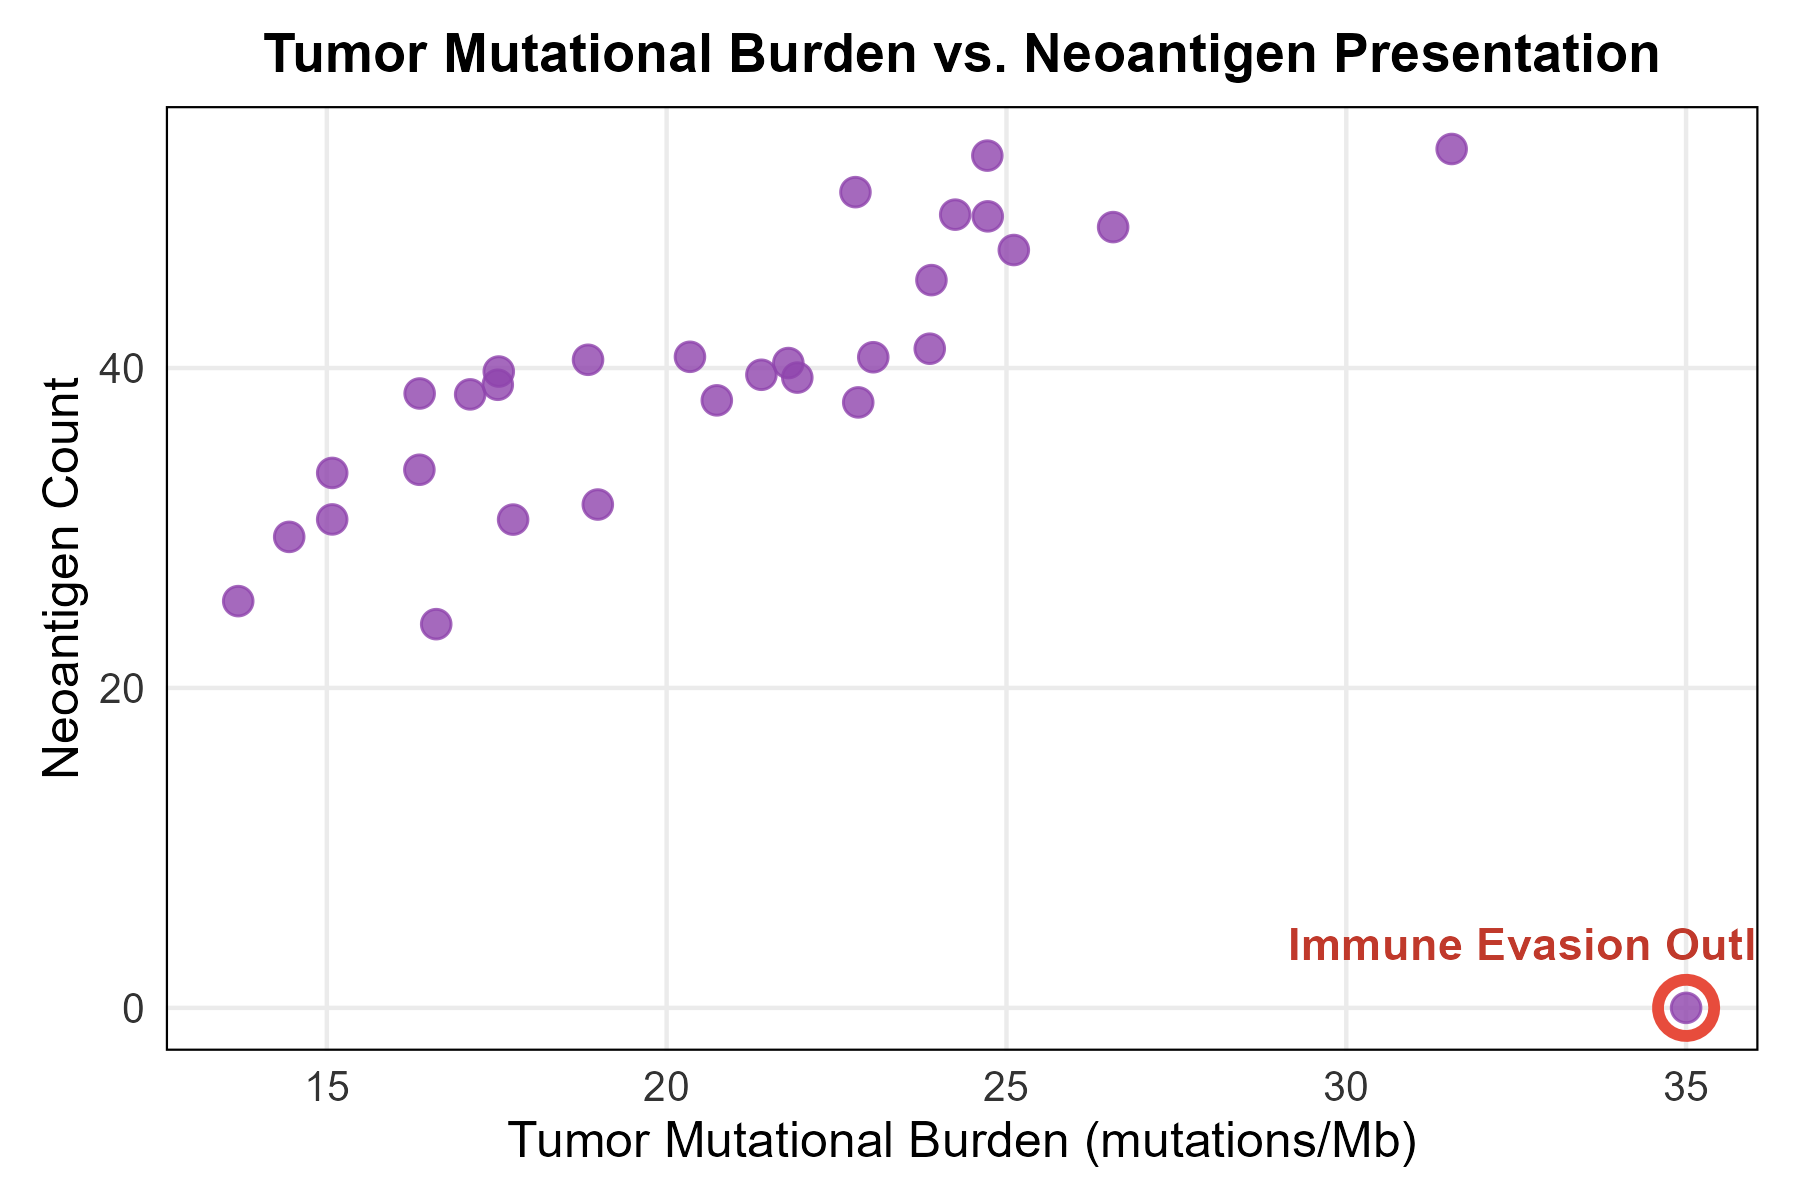
\includegraphics[width=\textwidth]{fig_ch3_outliers.png}
	\emph{Possible explanation:} A tumour may contain many mutations but still fail to present the resulting neoantigens effectively. For example, changes affecting the HLA antigen-presentation system could reduce what is displayed to the immune system.
\end{column}
\end{columns}
\end{frame}

% =============================================================
% PART III: EXPLORING ASSOCIATIONS
% =============================================================

% SLIDE 11
\begin{frame}{Exploring Associations}
  \begin{block}{Positive vs. Negative Association}
    \begin{itemize}
      \item Two variables are \textbf{positively associated} when above average values of one variable tend to accompany above average values of the other. 
      \item Two variables are \textbf{negatively associated} when above average values of one variable tend to accompany below average values of the other.
    \end{itemize}
  \end{block}
\end{frame}

% SLIDE 12
\begin{frame}{Example 3.8: Manatees and Powerboats}
\footnotesize
\begin{columns}[c]
\begin{column}{0.5\textwidth}
	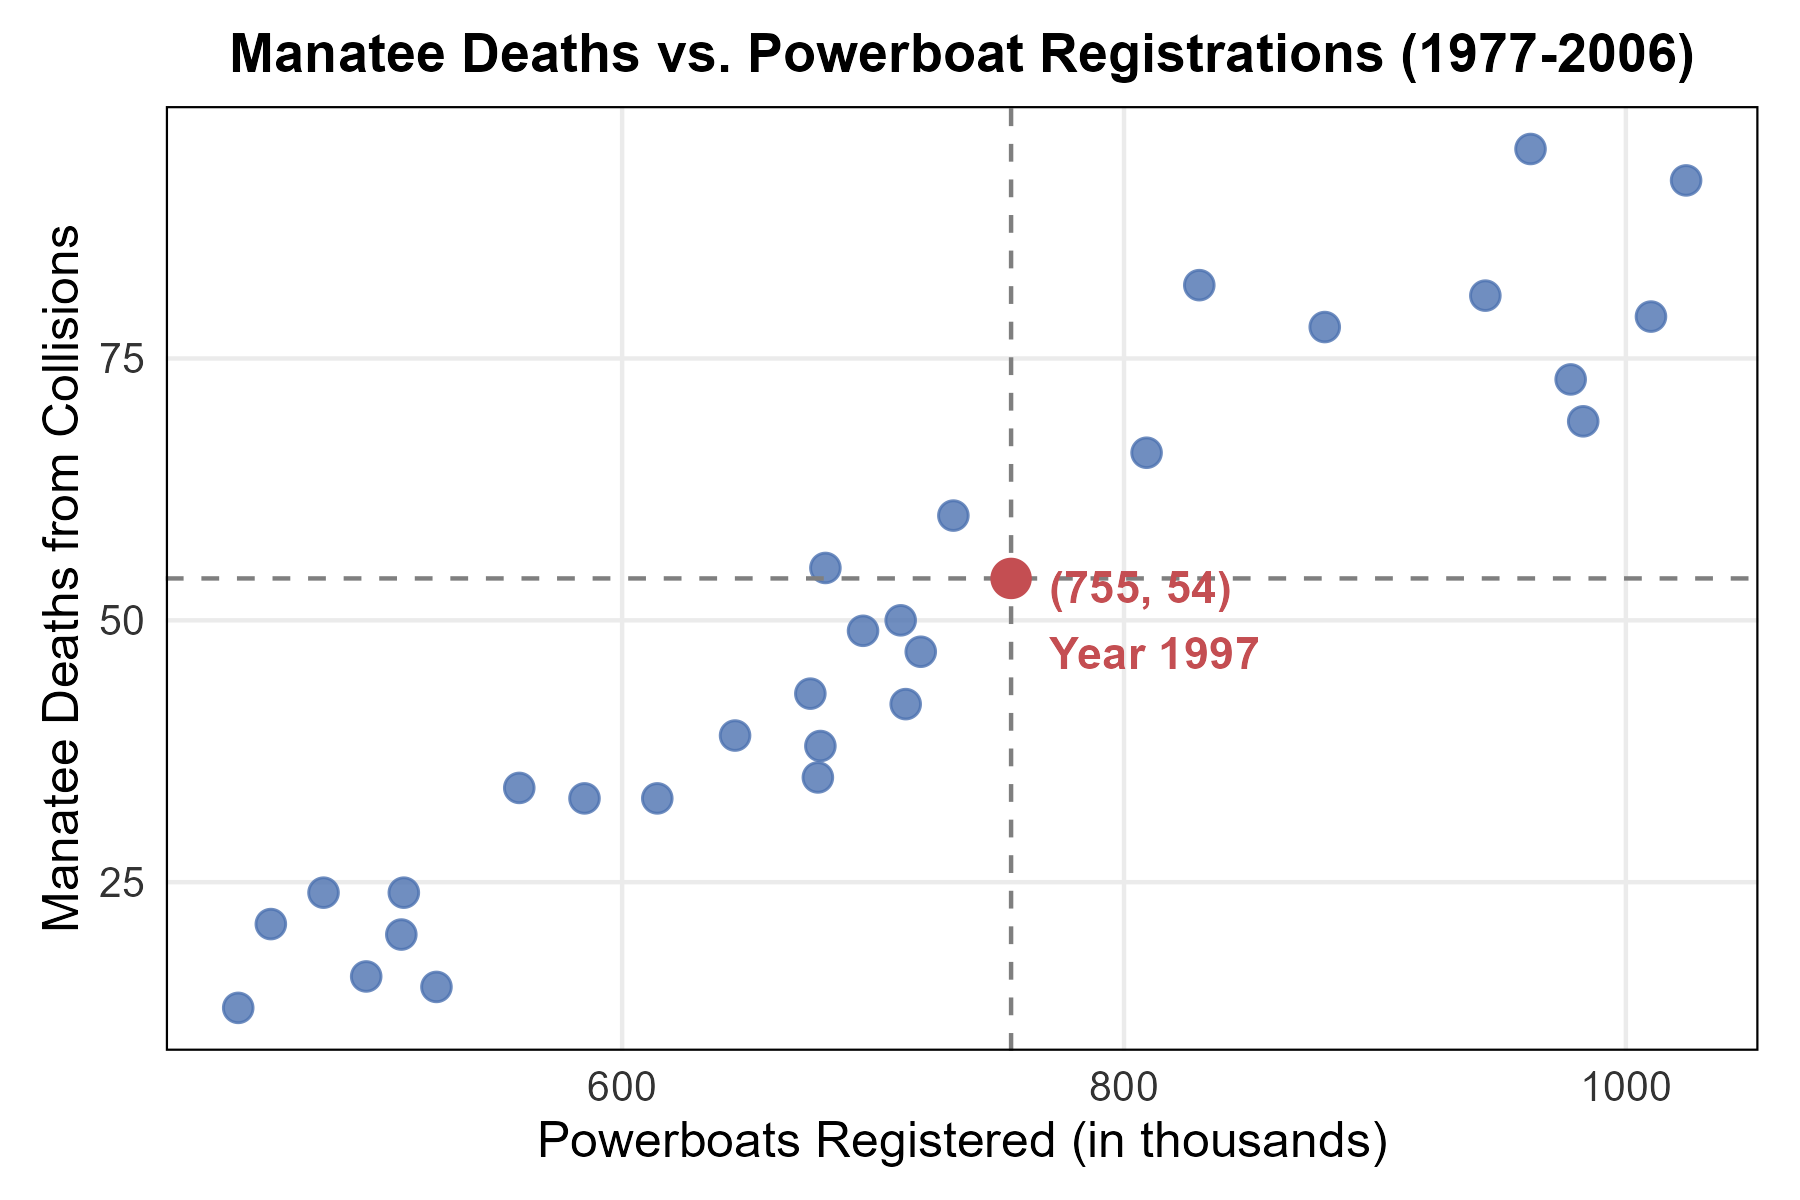
\includegraphics[width=\textwidth]{fig_ch3_manatees.png}
 \end{column}
\begin{column}{0.48\textwidth}
 \textbf{Context:} Researchers are studying whether increased boating activity is associated with the number of manatee deaths caused by collisions with watercraft in Florida. Each point represents one year of observations.
\begin{itemize}
	\item \textbf{Explanatory variable ($x$):} Number of registered powerboats in Florida
	\item \textbf{Response variable ($y$):} Number of manatee deaths caused by watercraft collisions
	 \item \textbf{Direction:} Positive. Years with more registered powerboats tend to have more manatee deaths.
	 \item \textbf{Form:} Approximately linear
	 \item \textbf{Strength:} Strong. The points follow the overall increasing pattern fairly closely.
\end{itemize}
\end{column}
\end{columns}
\end{frame}

% SLIDE 13:
\begin{frame}{Example 3.9: Does Fidgeting Keep You Slim?}
\footnotesize
\begin{columns}[c]
\begin{column}{0.48\textwidth}
\textbf{Context:} Researchers deliberately increased the food intake of a group of volunteers and measured how much body fat each person gained. They also measured changes in \textbf{Nonexercise Activity (NEA)}, which includes everyday movement such as walking, standing and fidgeting rather than planned exercise. Each point represents one volunteer.
\begin{itemize}
\item \textbf{Explanatory variable ($x$):} Change in Nonexercise Activity (NEA)
\item \textbf{Response variable ($y$):} Fat gain in kilograms
\item \textbf{Direction:} Negative. Volunteers with larger increases in NEA tended to gain less fat.
\item \textbf{Form:} Approximately linear\item \textbf{Strength:} Moderately strong. The points follow a decreasing pattern but show noticeable variation around that pattern.
 \end{itemize}
\end{column} 
 \begin{column}{0.5\textwidth}
	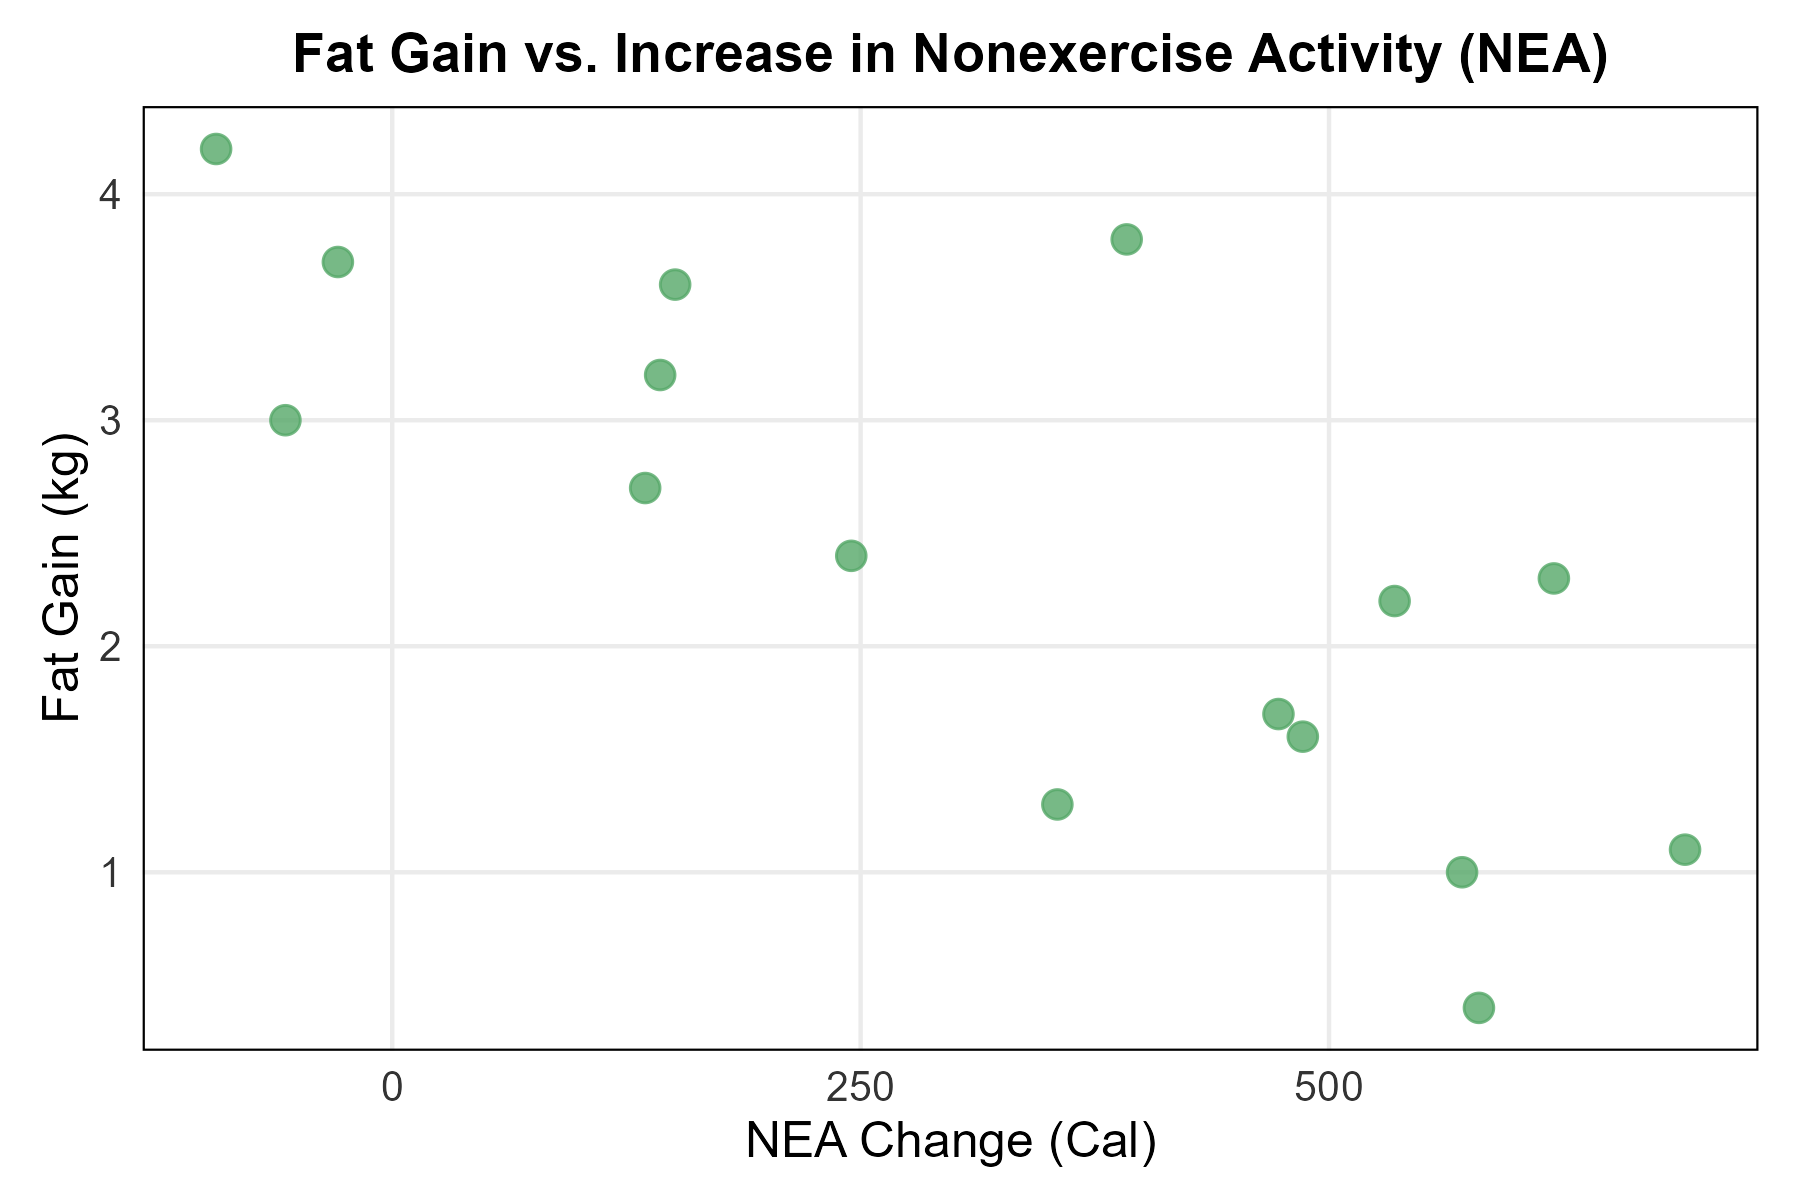
\includegraphics[width=\textwidth]{fig_ch3_nea_fat.png}
\end{column}
\end{columns}
\end{frame}

% SLIDE 14
\begin{frame}{Example 3.10: Magellanic Penguins}
\footnotesize
\begin{columns}[c]
\begin{column}{0.5\textwidth}
	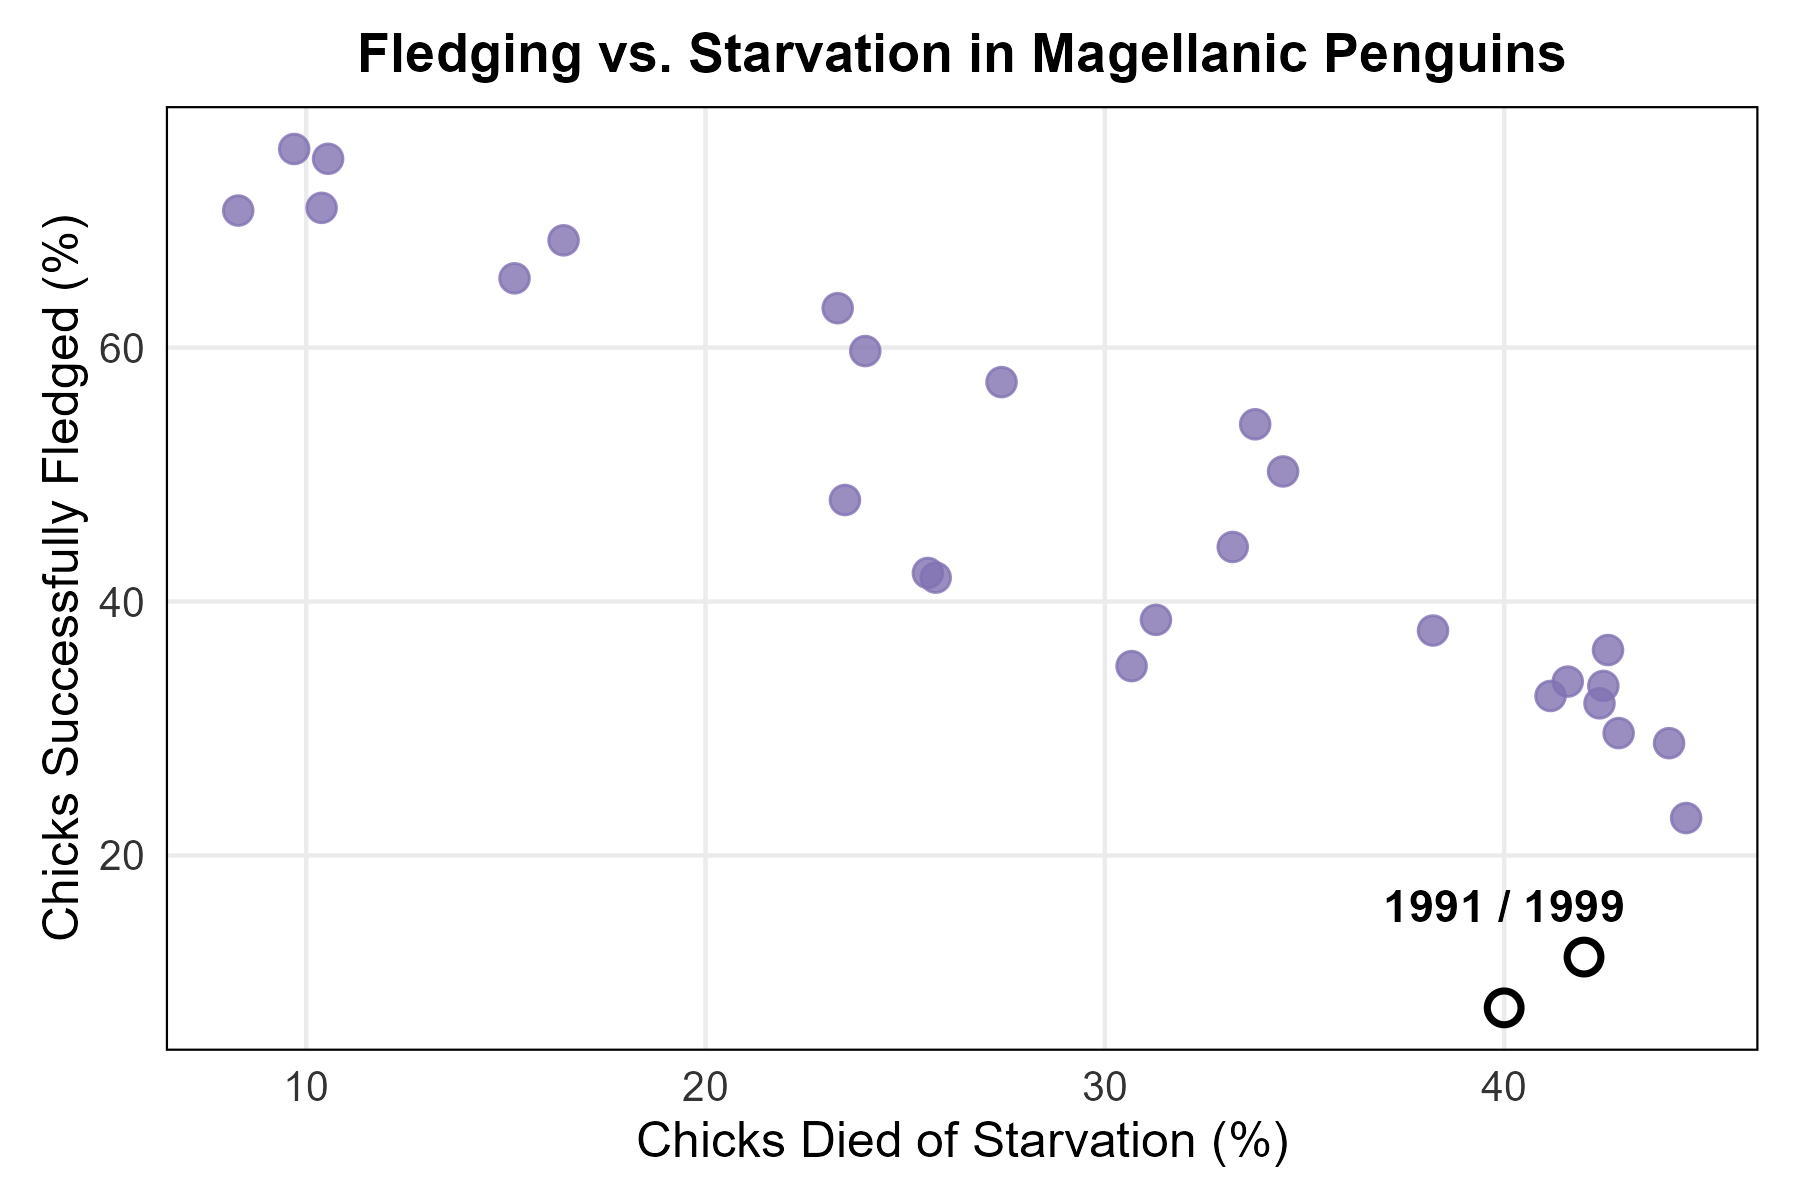
\includegraphics[width=\textwidth]{fig_ch3_penguins.png}
\end{column}
\begin{column}{0.48\textwidth}
\textbf{Context:} Researchers followed a colony of Magellanic penguins over many breeding seasons. For each year, they recorded the percentage of chicks that died from starvation and the percentage that successfully fledged, meaning that they survived long enough to leave the nest. Each point represents one breeding year.
\begin{itemize}
\item \textbf{Explanatory variable ($x$):} Percentage of chicks that died from starvation
\item \textbf{Response variable ($y$):} Percentage of chicks that successfully fledged
\item \textbf{Direction:} Negative. Years with more starvation generally had fewer chicks successfully fledging.
\item \textbf{Form:} Approximately linear
\item \textbf{Outliers:} The years 1991 and 1999 fall well below the overall pattern.
\end{itemize}
\end{column}
\end{columns}
\end{frame}

% =============================================================
% PART IV: CORRELATION (r)
% =============================================================

% SLIDE 15
\begin{frame}{Correlation ($r$)}
  Scatterplots rely on subjective visual judgment. To make reproducible claims, we need a mathematical summary. 
  \vspace{0.3cm}
  
  \textbf{Pearson's Correlation Coefficient ($r$)} measures the direction and exact strength of the \emph{linear} relationship between two quantitative variables.

  \vspace{0.2cm}
  The formula standardizes both variables (converting them into $z$-scores), multiplies them together and averages them:
  $$ r = \frac{1}{n-1} \sum \left( \frac{x_i - \bar{x}}{s_x} \right) \left( \frac{y_i - \bar{y}}{s_y} \right) $$
\end{frame}

% SLIDE 16
\begin{frame}{Crucial Properties of $r$}
  \begin{enumerate}
    \item $r$ is always a number strictly between $-1$ and $+1$.
    \item $r > 0$ indicates a positive linear association; $r < 0$ indicates a negative linear association.
    \item Values near 0 indicate a very weak linear relationship. Values near $-1$ or $+1$ indicate points that lie nearly exactly on a straight line.
    \item \textbf{$r$ only measures linear strength.} It is completely blind to curved/non-linear relationships.
  \end{enumerate}
\end{frame}

% SLIDE 17
\begin{frame}{Example 3.11: The Mechanics of Correlation (Frog Locomotion)}
A biologist measures the snout-vent length (cm) and maximum leap distance (cm) of 5 juvenile bullfrogs.
\vspace{0.3cm}
\begin{table}
\centering
\begin{tabular}{ccc}
\toprule
\textbf{Frog ID} & \textbf{Length $x$ (cm)} & \textbf{Leap Distance $y$ (cm)} \\
\midrule
1 & 4.0 & 32.0 \\
2 & 5.0 & 42.0 \\
3 & 6.0 & 48.0 \\
4 & 7.0 & 55.0 \\
5 & 8.0 & 65.0 \\
\bottomrule
\end{tabular}
 \end{table}

\textbf{Question:} What is Pearson's correlation coefficient between frog length and leap distance?
\end{frame}

% SLIDE 18
\begin{frame}{Example 3.11: Calculating Pearson Correlation}

\end{frame}

% SLIDE 19
\begin{frame}{Example 3.11: Calculating Pearson Correlation}

\end{frame}

% SLIDE 20
\begin{frame}{Example 3.11: Calculating Pearson Correlation}

\end{frame}

% SLIDE 21
\begin{frame}{Example 3.11: Calculating Pearson Correlation}

\end{frame}

% SLIDE 22
\begin{frame}{Example 3.11: Calculating Pearson Correlation}

\end{frame}

% SLIDE 23
\begin{frame}{Example 3.11: Calculating Pearson Correlation}

\end{frame}

% SLIDE 24
\begin{frame}{Example 3.11: Calculating Pearson Correlation}
\scriptsize
\textbf{Step 1: Calculate the means and standard deviations}
\[
	\bar{x}=6.0 \qquad \bar{y}=48.4
\]
\[
	s_x \approx 1.581 \qquad s_y \approx 12.542
\]

\textbf{Step 2: Standardize each observation}
\scriptsize
\begin{center}
\begin{tabular}{ccccc}
\toprule
$x$ & $y$ & $z_x=\dfrac{x-\bar{x}}{s_x}$ &
$z_y=\dfrac{y-\bar{y}}{s_y}$ & $z_xz_y$ \\
\midrule
4 & 32 & $-1.265$ & $-1.308$ & $1.654$ \\
5 & 42 & $-0.632$ & $-0.510$ & $0.323$ \\
6 & 48 & $0.000$  & $-0.032$ & $0.000$ \\
7 & 55 & $0.632$  & $0.526$  & $0.333$ \\
8 & 65 & $1.265$  & $1.324$  & $1.674$ \\
\midrule
 & & & \textbf{Sum} & $\mathbf{3.984}$ \\
\bottomrule
\end{tabular}
\end{center}

\textbf{Step 3: Substitute into the correlation formula}
\[
	r = \frac{1}{n-1} \sum z_xz_y = \frac{3.984}{5-1} \approx 0.996
\]

The correlation is approximately $r=0.996$. The data show a very strong positive linear association: longer juvenile frogs tend to have greater leap distances.
\end{frame}

% SLIDE 25
\begin{frame}{Example 3.11: Correlation Using Sums}
\scriptsize
This equivalent formula calculates correlation directly from the deviations from the two means:
\[
	r_{xy} =\frac{\displaystyle\sum_{i=1}^{n}(x_i-\bar{x})(y_i-\bar{y})}{\sqrt{\displaystyle\sum_{i=1}^{n}(x_i-\bar{x})^2}\sqrt{\displaystyle\sum_{i=1}^{n}(y_i-\bar{y})^2}}
\]

For the frog data
\[
	\bar{x}=6.0 \qquad\text{and}\qquad \bar{y}=48.4
\]
\begin{center}
\setlength{\tabcolsep}{4.5pt}
\renewcommand{\arraystretch}{1.08}
\begin{tabular}{rrrrrrr}
\toprule
$x_i$ & $y_i$
& $x_i-\bar{x}$
& $y_i-\bar{y}$
& $(x_i-\bar{x})^2$
& $(y_i-\bar{y})^2$
& $(x_i-\bar{x})(y_i-\bar{y})$ \\
\midrule
$4$ & $32$ & $-2$ & $-16.4$ & $4$ & $268.96$ & $32.8$ \\
$5$ & $42$ & $-1$ & $-6.4$  & $1$ & $40.96$  & $6.4$ \\
$6$ & $48$ & $0$  & $-0.4$  & $0$ & $0.16$   & $0.0$ \\
$7$ & $55$ & $1$  & $6.6$   & $1$ & $43.56$  & $6.6$ \\
$8$ & $65$ & $2$  & $16.6$  & $4$ & $275.56$ & $33.2$ \\
\midrule
\textbf{Sum} & & $0$ & $0$
& $\mathbf{10}$
& $\mathbf{629.20}$
& $\mathbf{79.0}$ \\
\bottomrule
\end{tabular}
\end{center}
\[
r = \frac{79.0}{\sqrt{(10)(629.20)}} = \frac{79.0}{79.322} \approx 0.996
\]

\end{frame}

% SLIDE 26
\begin{frame}[fragile]{Example 3.11: Correlation in R (Method 1)}
\begin{block}{Method 1: Using the Formula}
\scriptsize
\begin{verbatim}
length_x <- c(4, 5, 6, 7, 8)
leap_y <- c(32, 42, 48, 55, 65)

# Store the number of observations
n <- length(length_x)

# Convert the x-values to z-scores
z_x <- (length_x - mean(length_x)) / sd(length_x)

# Convert the y-values to z-scores.
z_y <- (leap_y - mean(leap_y)) / sd(leap_y)

# Calculate Pearson correlation coefficient
r_manual <- sum(z_x * z_y) / (n - 1)

r_manual

 [1] 0.995939
\end{verbatim}
\end{block}
\end{frame}

% SLIDE 27
\begin{frame}[fragile]{Example 3.11: Correlation in R Using Sums}
\begin{block}{Using the sum-of-deviations formula}
\scriptsize
\begin{verbatim}
length_x <- c(4, 5, 6, 7, 8)
leap_y <- c(32, 42, 48, 55, 65)

# Calculate deviations from the means
x_deviation <- length_x - mean(length_x)
y_deviation <- leap_y - mean(leap_y)

# Calculate the numerator
numerator <- sum(x_deviation * y_deviation)

# Calculate the two sums in the denominator
sum_x_squared <- sum(x_deviation^2)
sum_y_squared <- sum(y_deviation^2)

# Calculate Pearsons correlation coefficient
denominator <- sqrt(sum_x_squared * sum_y_squared)
r_sums <- numerator / denominator

r_sums
[1] 0.995939
\end{verbatim}
\end{block}
\end{frame}

% SLIDE 28
\begin{frame}[fragile]{Example 3.11: Correlation in R (Method 2)}
\begin{block}{Method 2: Creating a Custom Function}
\scriptsize
\begin{verbatim}
calculate_r <- function(x, y) {

  # Store the number of paired observations
  n <- length(x)

  # Standardize both variables.
  z_x <- (x - mean(x)) / sd(x)
  z_y <- (y - mean(y)) / sd(y)

  # Calculate and return Pearson's correlation
  return(sum(z_x * z_y) / (n - 1))
}

calculate_r(length_x, leap_y)

[1] 0.995939
\end{verbatim}
\end{block}
\end{frame}

% SLIDE 29
\begin{frame}[fragile]{Example 3.11: Correlation in R (Method 3)}
While it's important to understand the math, R has a built-in shortcut for calculating Pearson's correlation coefficient.
\vspace{0.3cm}
\begin{block}{Method 3: The fast way}
\begin{verbatim}
# In practice, you will simply use the cor() function:
cor(length_x, leap_y)
 [1] 0.995939
\end{verbatim}
\end{block}

\textbf{Interpretation:} An $r$ of roughly $0.996$ tells us there is a nearly perfect, positive linear relationship between a juvenile frog's length and how far it can leap.
\end{frame}

% SLIDE 30
\begin{frame}{Example 3.12: Calculating $r$ (Spatial Reproducibility)}
\scriptsize
\begin{columns}[c]
\begin{column}{0.48\textwidth}
\textbf{Context:} A research lab uses a spatial transcriptomics assay to measure gene activity in a tissue sample. To check whether the laboratory procedure gives consistent results, the same type of experiment is performed twice under similar conditions. For each of 500 genes, the researchers compare the measured expression level from Replicate 1 with the corresponding expression level from Replicate 2. Each point represents one gene.
\vspace{0.3cm}
\begin{itemize}
\item \textbf{Explanatory variable ($x$):} Gene expression measured in Replicate 1
 \item \textbf{Response variable ($y$):} Gene expression measured in Replicate 2
\item \textbf{Correlation:} $r=0.9696$
 \item \textbf{Direction:} Positive
\item \textbf{Strength:} Very strong linear association
\end{itemize}
\end{column}
\begin{column}{0.5\textwidth}
	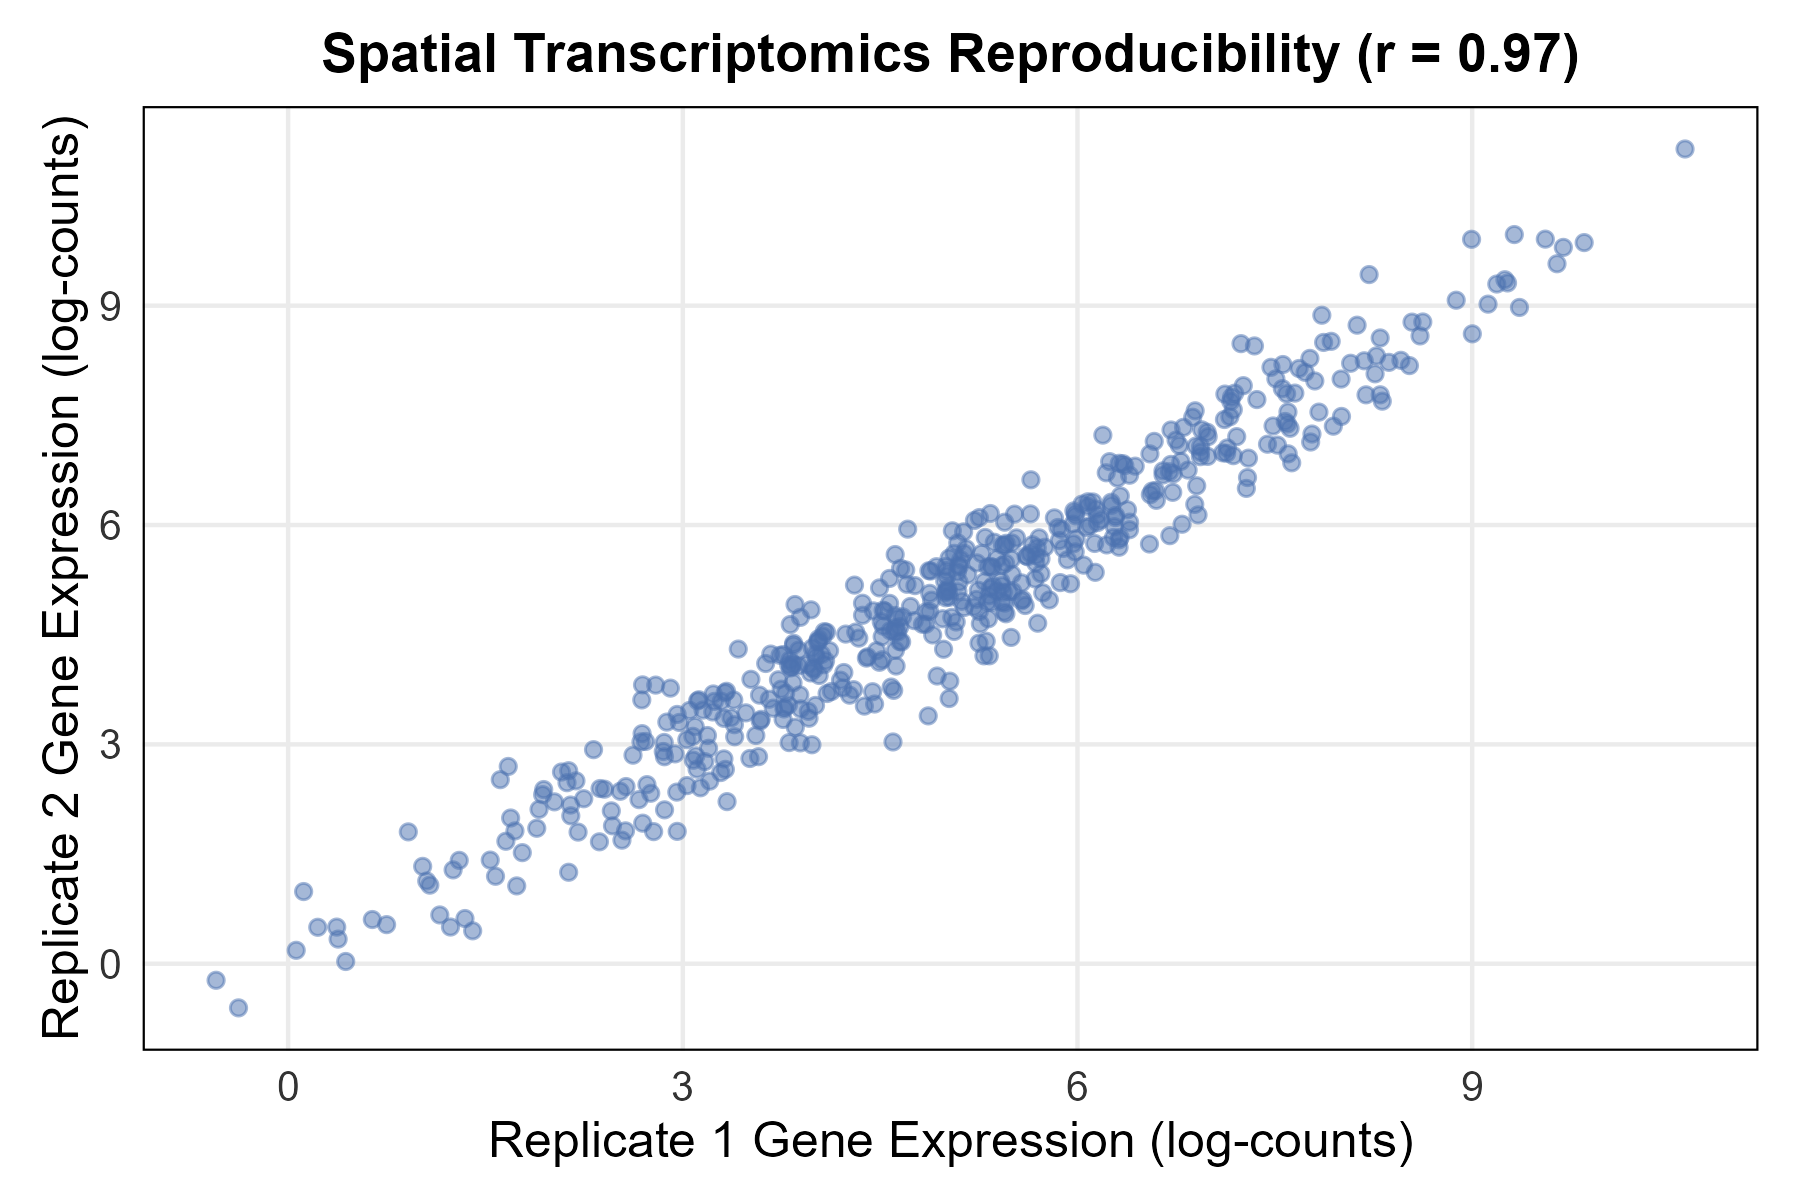
\includegraphics[width=\textwidth]{fig_ch3_reproducibility.png}
	\textbf{Interpretation:} Genes with higher expression in the first replicate also tend to have higher expression in the second replicate. The large value of $r$ suggests strong reproducibility of the relative gene-expression pattern.
\end{column}
\end{columns}
\end{frame}

% SLIDE 31
\begin{frame}{Example 3.13: The Unit-Independence of $r$}
Because the formula divides by standard deviations ($s_x$ and $s_y$), it entirely strips away the physical units of measurement. 
\vspace{0.3cm}
\begin{alertblock}{Rule}
Correlation has no units and changing the units of measurement does not change $r$.
\end{alertblock}
\vspace{0.3cm}
  
If you calculate correlation between swimming speed (\textbf{km/h}) and energy expenditure (\textbf{Kcal}), you get $r = 0.9424$. 
  
If a colleague converts the data to meters per second (\textbf{m/s}) and Joules (\textbf{J}), the correlation remains \textbf{identically 0.9424}. 
\end{frame}

% SLIDE 32
\begin{frame}{Example 3.14: The Non-Resistance of Correlation}
Remember that the mean ($\bar{x}$) and standard deviation ($s$) are non-resistant to outliers. 

\vspace{0.3cm}

Because the formula for $r$ relies entirely on $\bar{x}$ and $s$, \textbf{correlation is strongly non-resistant to outliers.} 

\vspace{0.3cm}

A single extreme point can completely destroy a strong correlation or artificially create one out of thin air! Let's look at a soil toxicology study.
\end{frame}

% SLIDE 33
\begin{frame}{Example 3.14: Heavy Metal and Root Length}
\footnotesize
\begin{columns}[c]
 \begin{column}{0.5\textwidth}
	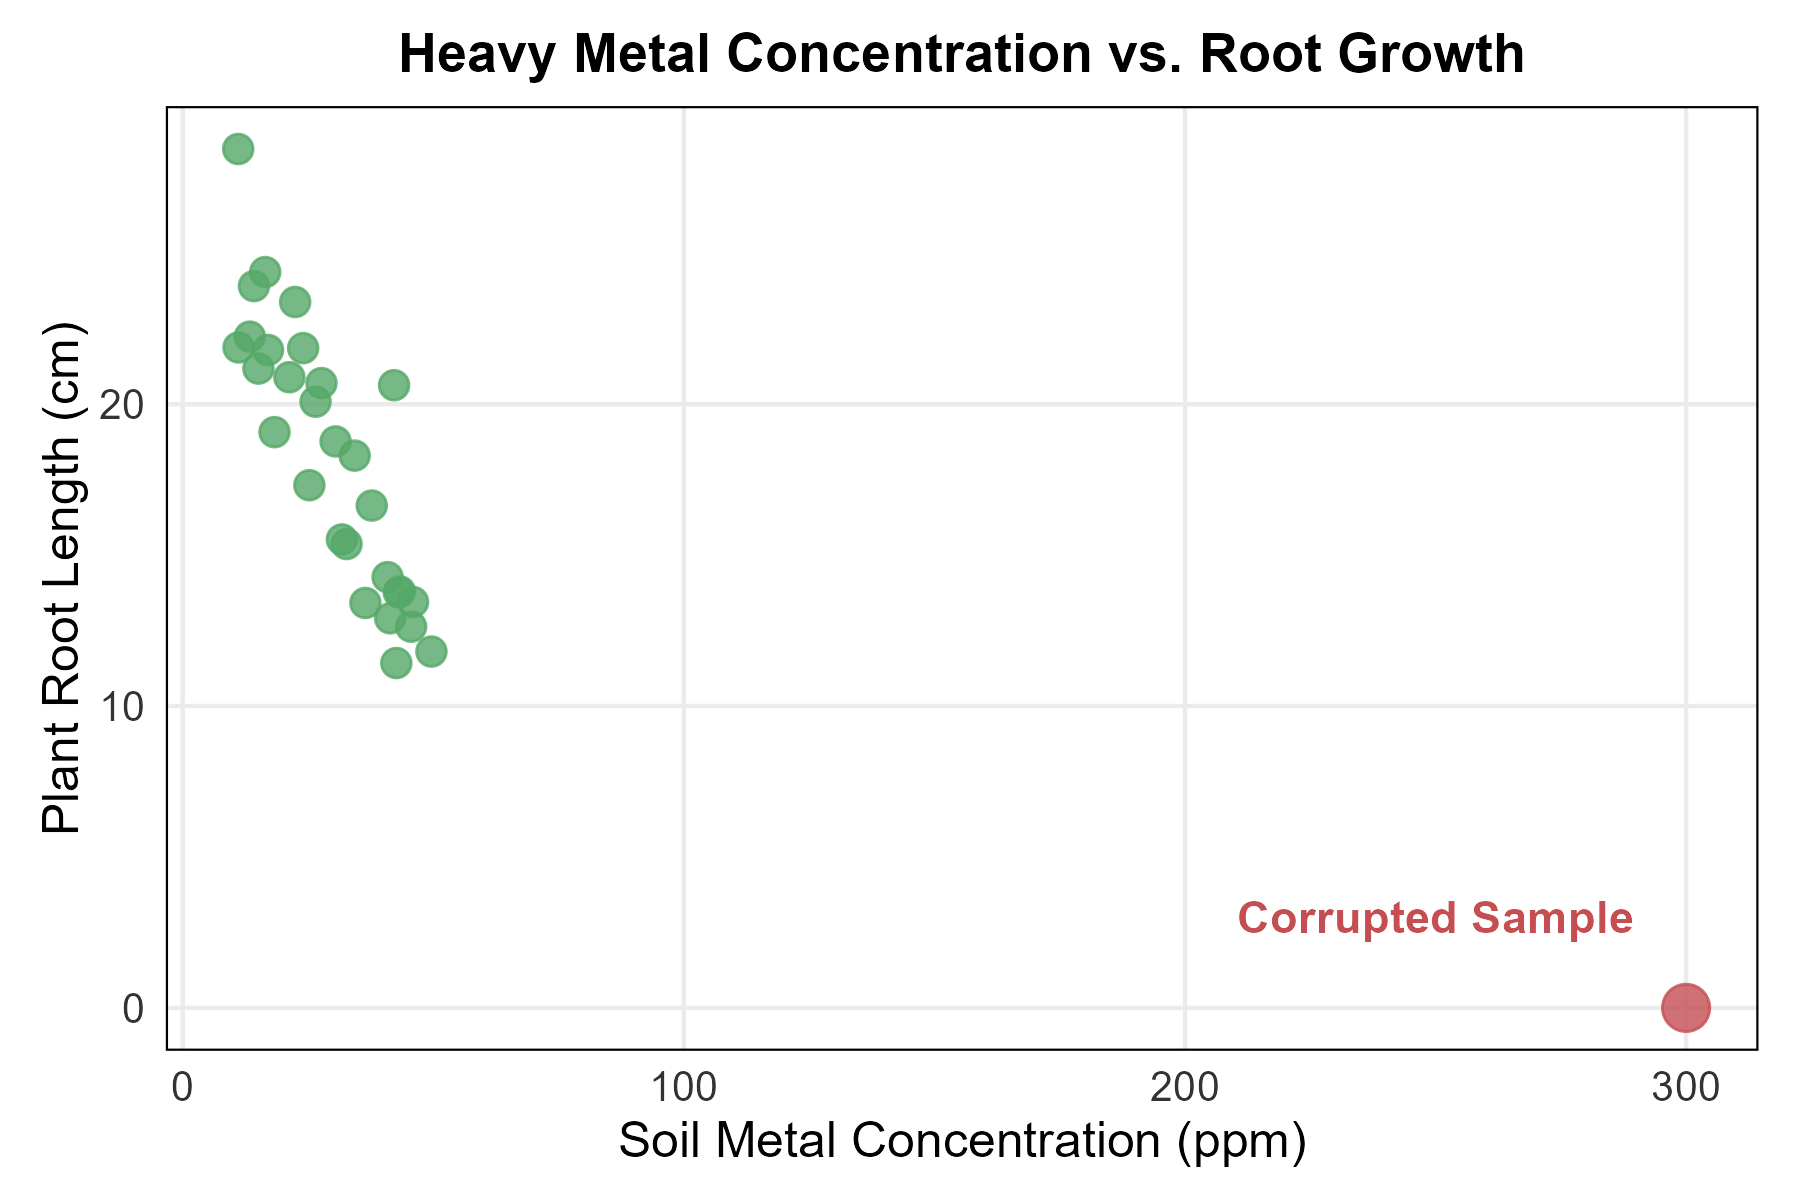
\includegraphics[width=\textwidth]{fig_ch3_toxic_outlier.png}
	One unusually extreme industrial sample was then included. Its metal concentration was far outside the range of the other observations and its root length was very small. After adding this one point, the correlation changes to approximately $r=-0.95$.
\end{column}
\begin{column}{0.48\textwidth}
\textbf{Context:} Researchers are studying whether higher concentrations of a heavy metal in soil are associated with reduced plant root growth. For each soil sample, they record the heavy metal concentration and the root length of a plant grown in that soil. Each point represents one soil sample.
 \vspace{0.2cm}
\begin{itemize}
	\item \textbf{Explanatory variable ($x$):} Heavy metal concentration in the soil
	\item \textbf{Response variable ($y$):} Plant root length
	 \item \textbf{Original pattern:} The 29 regular samples show a moderately strong negative linear association with $r=-0.77$
\end{itemize}
\end{column}
\end{columns}
\end{frame}

% SLIDE 34
\begin{frame}[fragile]{Summary of R Commands (Chapter 3)}
  Here are the key functions introduced in this chapter for bivariate analysis:
  \vspace{0.3cm}
  \begin{table}
    \centering
    \begin{tabular}{lp{8cm}}
      \toprule
      \textbf{R Command} & \textbf{What it Calculates} \\
      \midrule
      \texttt{length(x)} & Returns the number of elements ($n$) in a vector. \\
      \addlinespace
      \texttt{sum(x * y)} & Multiplies two vectors together element-by-element, then sums the result. \\
      \addlinespace
      \texttt{function(x, y) \{...\}} & Allows you to create your own custom, reusable mathematical formulas. \\
      \addlinespace
      \texttt{cor(x, y)} & Calculates Pearson's Correlation Coefficient ($r$) between two variables instantly. \\
      \bottomrule
    \end{tabular}
  \end{table}
\end{frame}


\end{document}